% !Mode:: "TeX:UTF-8" 

\BiChapter{绪论}{Introduction}\label{chap1}

%本章对 \LaTeX{} 排版系统做一个简要介绍,希望没有使用过 \LaTeX{} 的同学对 \LaTeX{} 有一个初步认识。

%=========================================================================================
\BiSection{研究的背景}{Background}\label{chap11}
\BiSubsection{研究的意义}{Motivation}\label{chap111}

%参考线性系统理论第一章的叙述方法,先要定义清楚研究对象。等等。。再看本文是否也能按照更好的方式叙述。

21世纪的新20年,网络正以前所未有的速度越来越紧密地参与到民生社会中,为满足国家民生需求、新基建拉动内需和产业升级起到了至关重要的作用。从“百度一下”到网红全民直播带货,从实现“三网通”到发展“新基建”的国家战略,小到优化社会资源效率的办公数字化,大到勾勒出智能交通、智慧城市和万物互联的5G海洋,无一不是构建在网络基础设施的快速发展之上。思科公司预计,到2023年全球家用互联网总带宽将达到$5.85$Ebps\footnote{1 Ebps=$10^6$Tbps=$10^{18}$bps} (是现在的3.27倍),移动互联网用户预计达到57亿,其总流量可达$11.3$Ebps (将达到目前的5倍),其中5G流量将占据移动互联网总带宽的76.5\%(0.6\%,2019年)\citeup{huawei2019,cisco2019}。由于深度学习、AI、大数据、云计算、物联网的快速发展\citeup{gubbi2013internet,hashem2015rise},这些新技术将催使新零售、新金融、新医疗、新教育、新制造、云视频和云游戏等行业“云化”,海量的数据会在数据中心内部服务器间网络以及外部网关中传递,这些关键应用将会改变数据中心算力构成和数据中心内部网络结构特性。

IDC报告称,2019上半年中国公有云服务整体市场(Iaas/PaaS/SaaS)达到54.2亿美元,并预计在未来5年间内以年均复合46\%的速度快速增长\citeup{idc2019,idc2020}。数据中心内服务器计算力呈现异构化趋势,GPU,AI芯片,FPGA等使用非通用类型指令集和特殊体系架构计算单元已成为目前分布式计算领域的热点话题。现在超大型数据中心一般可容纳数十万台终端服务器,内部网络链接数量多、拓扑规模大、传送海量数据,这使得现有的网络变得异常复杂\citeup{hong2018b4,singh2015jupiter,mckeown2008openflow,casado2007ethane}。同时,新的数据包类型层出不穷也使传统网络显得不够灵活。

为应对以上挑战,最近十年以来网络技术和架构经历了快速演进和变革,数据中心网络尤为明显\citeup{li2019hpcc,singh2015jupiter,alizadeh2010data,wu2012tuning}。传统网络下,为增强交换机的扩展能力,二层网络增加了广播、桥接等复杂功能。这种网络架构在小规模应用时可以展现强大的智能性与可扩展性,但当网络规模进一步增加,网络中容易出现广播风暴、链路收敛慢等一系列问题。现代的大型网络设计中无需使用这类复杂的离线交互协议。事先规划好网络拓扑结构,只保留三层以上的功能,在各个层次之间的网络设备功能也逐步变得统一透明。设备统一化有助于降低网络部署的复杂度。研究人员通常需要持续进行网络测量、监控、容错、提升效能的工作。由于思想的创新和技术的推进,设备厂商不断开发出具备各种高级功能的交换芯片。硬件功能强大的同时,复杂的网络管理也遇到新的挑战。

为解决设备制造复杂和设备管理复杂的问题,软件定义网络(Software Defined Network,SDN)概念的提出拨开了迷雾。SDN将数据平面和控制平面解耦。在数据平面上,对数据包的处理统一做查找-转发(Match-Action)抽象。控制平面负责建立网络拓扑,控制并下发流表。这样所有的数据包转发行为都由控制平面的软件逻辑管理,数据平面需要支持任意一种网络协议。由于软件具有强大的灵活性以及开发的敏捷性,SDN大大加速了网络创新和智能化管理的进程。数据平面和控制平面的通讯桥梁由符合OpenFlow协议的安全通道(Secure Channel)构成。因此数据平面统一化、简单化,使得网络交换设备向白盒化方向发展。	

大规模网络无论在底层设备架构还是运维方式上仍没有停止变革的脚步,这为可编程硬件的发展带来了巨大空间。随着云服务概念和大规模机器学习的落地,近年来以云计算为代表的数据中心网络规模指数增长。网络功能虚拟化在数据中心内部是关键一环,虚拟交换机则是主机内各虚拟机之间数据包转发的核心软件。随着众核CPU架构快速发展,服务器内虚拟机布置资源大幅扩张,促使主机出口吞吐量从40GbE向100GbE甚至400GbE演进。不但如此,复杂的网络安全规则、流量监控等功能模块进一步吞噬了大量CPU资源。研究人员需要花费大量时间去解决虚拟化网络环境下的大规模扩展方案,创新变得异常艰难。x86架构的CPU适合于处理灵活多变的计算和控制任务,对于做重复、流式的数据处理并不能获得最优效率,厂商往往不得不依靠部署大量服务器来解决网络问题。

为缓解网络对CPU消耗过大,业界提出一种基于智能网卡的解决方案。智能网卡采用网卡芯片(ASIC)、FPGA、网络处理器、ARM等器件,在网卡端形成新的算力集合,目标为提高流式计算的效率。可以把对数据包的转发操作、网络安全规则检查等功能从主机端转移下来。ASIC具有最好的性能和最高的能量效率,但每次重新部署消耗的研发资金和周期都过长。对于运营商,由于快速发展的网络架构,设备的更新换代周期变短,如何优化设备、仪器等一次性支出(Capital Expenditure,CapEx,资本性支出)也会成为在探索新型网络架构时重要的参考因素。

随着创新需求的进一步提高,只有让底层硬件拥有灵活的可配置能力才能满足目前行业变革的需求,研究人员提出了数据包处理编程协议无关(Programming Protocol-Independent Packet Processors,P4)概念。P4不但支持SDN网络控制和管理特性,还提出了数据平面可编程的概念。数据包在数据平面内的处理模型遵循解析-查找-匹配的抽象模式。P4同时规范了一种编程语言\citeup{p4},它可以控制数据平面对数据包的任意解析行为,也可以自由配置查找表的数据位宽和多级流表之间的查找流水线\citeup{rmt,mswitch}。这种更高阶的硬件编程模型使交换设备更加透明,设备与网络协议解绑。除此之外,网络端到端的大带宽、低时延需求引申出了网络功能硬件卸载、网络随路计算等概念,这也进一步促使网络面向全面可编程化方向发展。

综上所述,现代网络在向软件定义、数据平面可编程的方向发展。网络架构变迁的核心是有一套可编程的可以映射上层控制逻辑的硬件数据平面。本文主要探索可编程硬件的网络系统,使其能够满足快速迭代的网络创新需求,在能够提供与现阶段匹配的处理性能的同时兼顾系统安全性。

\BiSubsection{技术简介}{Technology Brief}\label{chap112}

软件定义网络的基本设计概念是将数据平面与控制平面分离\citeup{mckeown2008openflow,ethane}。其中网络数据平面完成计算机之间通信数据包的匹配、修改、传送、转发的软硬件设备。数据平面的可编程性要求网络管理员拥有对数据平面的各个特性做快速个性化定制的能力。网络的控制平面维护全网视野、调度、配置针对流的转发条目。运行在控制平面内的各种应用构成了其全部功能。当前SDN网络系统设计架构如图\ref{fig:sdnarcs}所示,主要有软件方法实现,专用硬件实现和新型可编程硬件。

\begin{figure}[!ht]
	\centering
	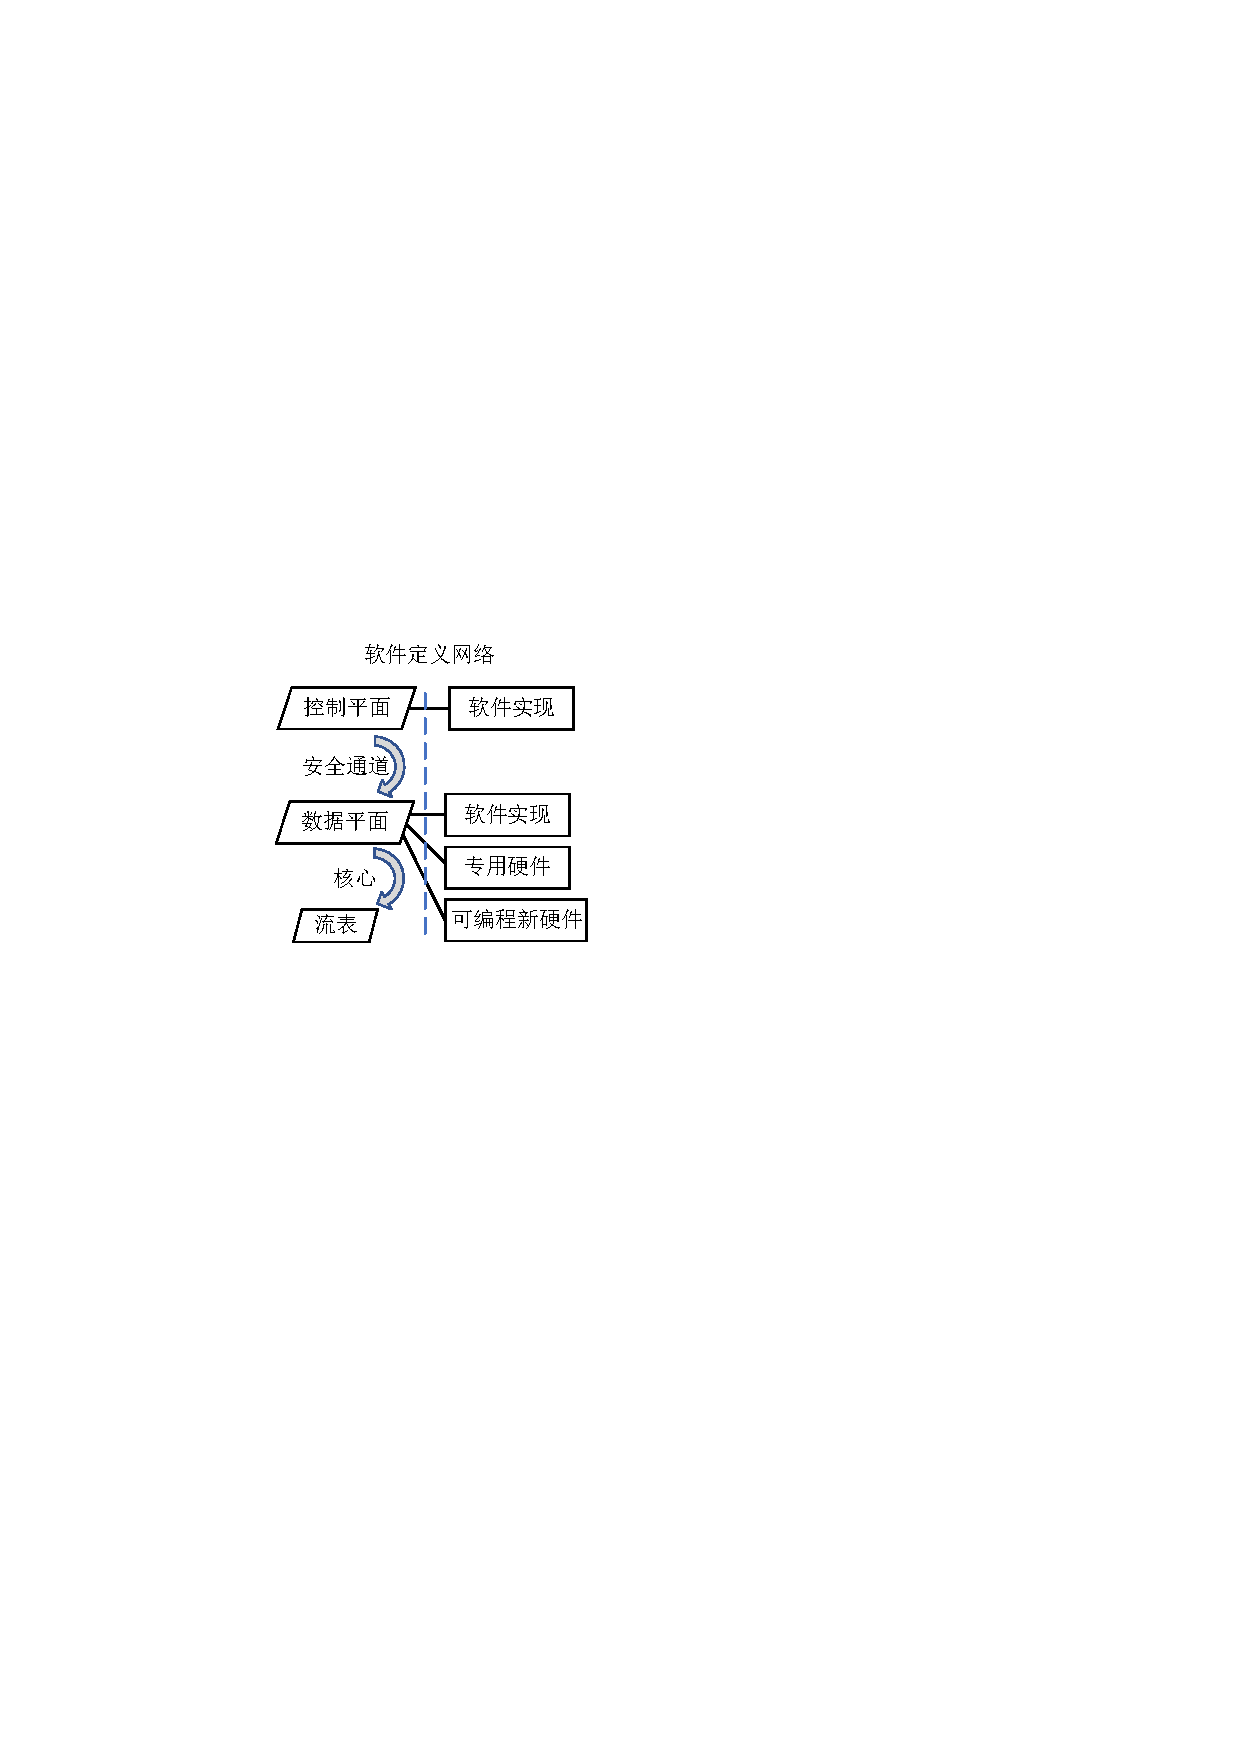
\includegraphics[scale=1]{sdnarcs.pdf}
	\caption{软件定义网络结构及其实现方案} \label{fig:sdnarcs}
\end{figure}

在不同场景下,网络对数据通信的需求千差万别,根据应用场景流量大小不同、处理过程复杂程度来设计选取数据平面的实现方案。本文在第\ref{sec:pdpintro}章详细介绍各类数据平面的实现方案的优缺点,并着重于各类数据平面可编程性的分析。目前最主要的两类数据平面是“软件交换机”和“专用硬件交换机”。两者在功能上都能够对数据包做一系列处理,包括匹配、查找、统计、传送、转发和安全校验等,其中“流表”是实现数据平面功能的核心函数(器件)。数据平面包含一个可以与远端控制器沟通的代理机构,这部分功能着重于协议通信以及安全通道信息加解密,主要由轻量级处理器构成。硬件交换机之于软件交换机的主要区别在于处理数据包的性能以及交换容量。数据包处理性能主要参数为吞吐量(字节每秒)和包吞吐量(包每秒)。目前基于软件实现的数据平面性能可达到60Gbps/60Mpps\citeup{pisces}。当数据包处理复杂度(操作步骤数量)增加时,软件交换机的性能会大幅下降。专用硬件交换机有接口数目多、交换容量大的特点,一般能满足64个100G端口的总交换容量。而且硬件交换机转发时延低,性能与数据包处理步骤数目几乎无关,稳定性良好。在核心网络和高性能网关等领域主要使用基于硬件的交换设备,但成熟设备功能固定、更换成本高,如果需要更新网络功能,几乎无所适从。所以目前在数据中心网络的NFV(网络功能虚拟化)等场景内,软件交换机依然占据很大份额。由于软件交换机灵活性高,开发人员能够快速迭代部署新功能,且传统单机通信速率需求不高,软件交换机尚能满足需求。但随着人工智能、5G领域的发展,数据中心网络内通信容量需求快速增长,转发时延收紧,软件交换机性能瓶颈凸显。运营商不得不为网络任务大量堆叠服务器。本文主要侧重于研究服务器和核心交换网络中,如何使用可编程硬件来大大缓解网络性能瓶颈。针对控制平面,本文使用SDN全局优化的思想,实现对网络中的瓶颈资源(如流表资源)的可扩展性并提升通信协议的安全性。

\BiSubsection{国内外应用与研究现状}{Application and research status}\label{chap113}

为增强数据平面的可编程性以及缓解基于硬件交换设备流表资源不足的现状,工业界学术界互相促进、广泛研究并提出了多种方案。

1)基于软件的数据平面

这类技术着重于便捷开发,价格低廉,无需在网络中部署专用设备的场景,是快速实现功能的首选方案。目前在虚拟化的云服务系统中,已经部署了大量基于软件的网络功能:(1)转发层,华为CE1800V\citeup{huawei1800v}是专为数据中心云计算虚拟化环境部署的一种分布式虚拟交换机。其支持标准Open Flow1.3控制协议,以及Open vSwitch 数据库管理协议(OVSDB),基于英特尔DPDK(Data Plane Development Kit)技术提供每核12Gbps的转发吞吐,比业界平均水平高出20\%。(2)流量监管,Activelogic\citeup{activelogic}是一个提供安全可靠、流量分类、提高QoE(Quality of Experience)能力的网络管理工具。它基于软件可自动化部署,依靠超大规模、人工智能技术以及云计算场景优化的能力,在数据平面解决流量监管的问题。基于软件的数据平面功能可以依靠堆叠CPU核数来实现大规模的性能扩展,但由于计算复杂度过高、基于指令的图灵机在高速内存共享和海量数据处理场景中效率低下,即使简单转发的性能达到100Gbps线速也需要占用10个CPU核心\citeup{pisces,v580}。综上所述,单纯地依靠软件处理器扩张来增加网络性能边界收益将越来越小。

2)基于白盒交换机和P4专用芯片的数据平面

硬件交换机在网络性能方面大幅超越基于通用软件服务器的数据平面\citeup{p4,v580}。符合OpenFlow规范的白盒交换机可将控制平面移交给远端软件层,从而实现设备的再开发能力。在DDoS防护、负载均衡等基础网络转发设备的智能化和可定制化方面给出了比较好的灵活性。阿里巴巴在其云计算网络场景中,通过可编程硬件交换机和通用服务器结合来实现公有云的网关服务。此架构既拥有芯片带来的网络转发性能提高(6.4Tbps,400ns延迟)也具有可编程带来的网络功能快速部署迭代能力,还能实现软件所擅长的复杂网络调度功能\citeup{alibaba}。这样同时兼顾了性能、灵活性,在大规模扩展网络体系结构时达到降低成本,满足业务需求和简化网络架构同时提升服务稳定性。数据平面可编程芯片提供了硬件层面上的可编程包头抽取器、可编程流表以及可编程执行器。其依靠快速查表(TCAM,SRAM)法,或经过后期编程选取特定的冗余逻辑模块(在ASIC芯片内部的空间上堆叠的可编程单元)法,来完成专用电路(ASIC)的直接逻辑描述\citeup{rmt,tofino2}。不过这类可编程芯片架构提供的可编程性也不是完备的,可编程流表限制了查找的宽度、深度范围,造成了逻辑资源浪费以及流水线处理时延较大。同时,ASIC设计定型之后无法增加新的用户特性(状态转发、随路计算、监测计数和包调度特性),导致这类P4专用芯片的可编程范围是大大受限的。

3)基于FPGA的自主设计的数据平面

现场可编程门阵列(FPGA)是一种灵活性可以与软件媲美可编程硬件,性能和效率与专用硬件接近。现代高速云架构依赖于每个专用硬件(ASIC)网络节点的支持,随着网络功能需求多变与复杂化,ASIC类型的网络处理芯片并不能解决所有可编程场景需求。业界已经开始将网络堆栈向基于FPGA的网卡中卸载\citeup{serverswitch,azure,yan2016all}。为了推广可编程硬件,学术界牵头推出了基于FPGA的智能网卡开源项目NetFPGA\citeup{netfpga2014},龙头企业Xlinx、Intel等也纷纷推出了基于MPSoC/FPGA的自适应计算加速平台Alveo\citeup{xilinx,alveo}系列智能网卡和N3000\citeup{intelfpganic}系列网卡。目前,基于FPGA的可编程数据平面已经广泛应用在5G接入边缘网络\citeup{intel5g}、数据中心计算存储\citeup{xilinxnvme}、核心网络低延迟加速器\citeup{intelgre}以及高性能高可靠性高安全性的数据中心防火墙\citeup{intelddos}加密通信\citeup{intelencryption}等领域。FPGA一般用硬件描述语言Verilog、VHDL等开发。一个合格的硬件工程师的培养周期要远大于软件工程师,这也是目前网络领域硬件卸载最难所在。为了解决这种不足业界也推出了类似C语言的高层次综合工具(HLS\citeup{xilinxhls})。但使用这类工具必须学习1000多页的开发文档\citeup{hlsdoc},而且并不是所有代码都可以直接被工具转译,(1)也需要考虑硬件细节,合理修改设计以降低FPGA内部资源消耗;(2)需要自主决定并行区块;(3)需要在代码中融入这种编译器的特性标记字符。总体来看并没有从本质上改善对硬件编程的困难程度。除此之外,由于在FPGA中复杂逻辑对并行总线宽度的频率敏感度高,一个大型工程时序逻辑的处理主频一般不会超过200MHz。即使每个时钟节拍都可以处理一个数据包,那么FPGA流水线在处理最小包时的最高吞吐量也只有134Gbps\footnote{134Gbps=200Mpps*(64+20)*8bits},这对FPGA应用在核心网包交换场景形成了瓶颈。

4)改善数据平面内流表资源匮乏

高性能内部需要使用基于硬件的高速缓存(如,TCAM,SRAM等)来进行查表操作。带有掩码功能的查找表(TCAM)是做IP最长前缀查找的高性能核心部件。TCAM具有单周期吞吐的流水线掩码查找能力使得其功能难以由一般存储器代替。但其价格以及能源消耗都较大,基于TCAM的流表容量通常都比较小,且极有溢出的可能。
流表溢出会导致交换机转发性能降低,甚至会导致数据平面与控制器通信报文数量爆炸增长,给SDN控制器的安全造成隐患\citeup{qsy2018openflow}。
在解决此类问题时,研究人员一般从以下两方面着手:(1)提升流表项数量。当TCAM存储容量固定时,假设宽度为key、深度为depth,二者的乘积恒定。显然如果可以降低流表项宽度值key,可以变相增加流表项数量。在数据中心网络场景下,可以通过重新定义包头域宽度来定义流,无需使用现有过宽的包头域。例如将所有流映射到16bits宽度的匹配域,可增加流表项容量10倍左右,等数据包离开网关时在将原始包头还原\citeup{kannan2013compact}。但这种思路仅仅在内网有效,而应对如今更大流量的骨干网,核心网显然无所适从。(2)提高转发设备流表的更新速度。表项替换分为两步,首先控制器选择一条已有表项并删除,之后控制器发送并新增一条表项。一些算法可对TCAM存储空间进行优化合并,但多个表项之间会产生依赖\citeup{meiners2011bit}。若希望删掉一条逻辑表项,会牵扯大范围的物理存储内容,这增加了修改表项时的操作复杂度,也使得更新表项速度变慢。若流表项剩余空间足够,新增表项可以直接写入空白区域而不去更改已有内容。还可以在运行时检测流表命中频次,提前探测并删除“死流”,为表项争取最大的可用空间\citeup{kannan2014flowmaster}。存储分级是一种通用的应对策略,例如使用TCAM+SRAM的双表查询,可大幅度扩展流表数目。考虑到SRAM对带掩码表项资源利用率低,查找速度慢,一般只能将老鼠流存放入SRAM空间,实际应用范围比较窄。
以上方法的核心思想是增加表项的原有表项空间,其只能拖延溢出的发生时间,对缓解流表溢出造成通信质量下降以及控制消息爆炸等危害依然无效。

\BiSection{研究内容}{research content}\label{chap12}

本文主要探索基于可编程硬件的高性能网络数据平面,对主机侧网络和交换层网络的数据平面实现加速,并研究在软件定义网络(SDN)概念下控制平面对全网核心流表资源的全局优化方法。如图\ref{fig:proghardwarePDParcs}所示,首先,论文把基于软件的网络高性能存储需求和密集型计算功能向网卡硬件卸载。其次,利用FPGA与交换芯片使能交换网络数据平面的高性能高可编程性。第三,流表是基于硬件的高性能数据包转发的核心资源,本文基于软件定义网络控制面数据面分离的特点,对数据平面的流表资源进行了全局优化。

\begin{figure}[!ht]
	\centering
	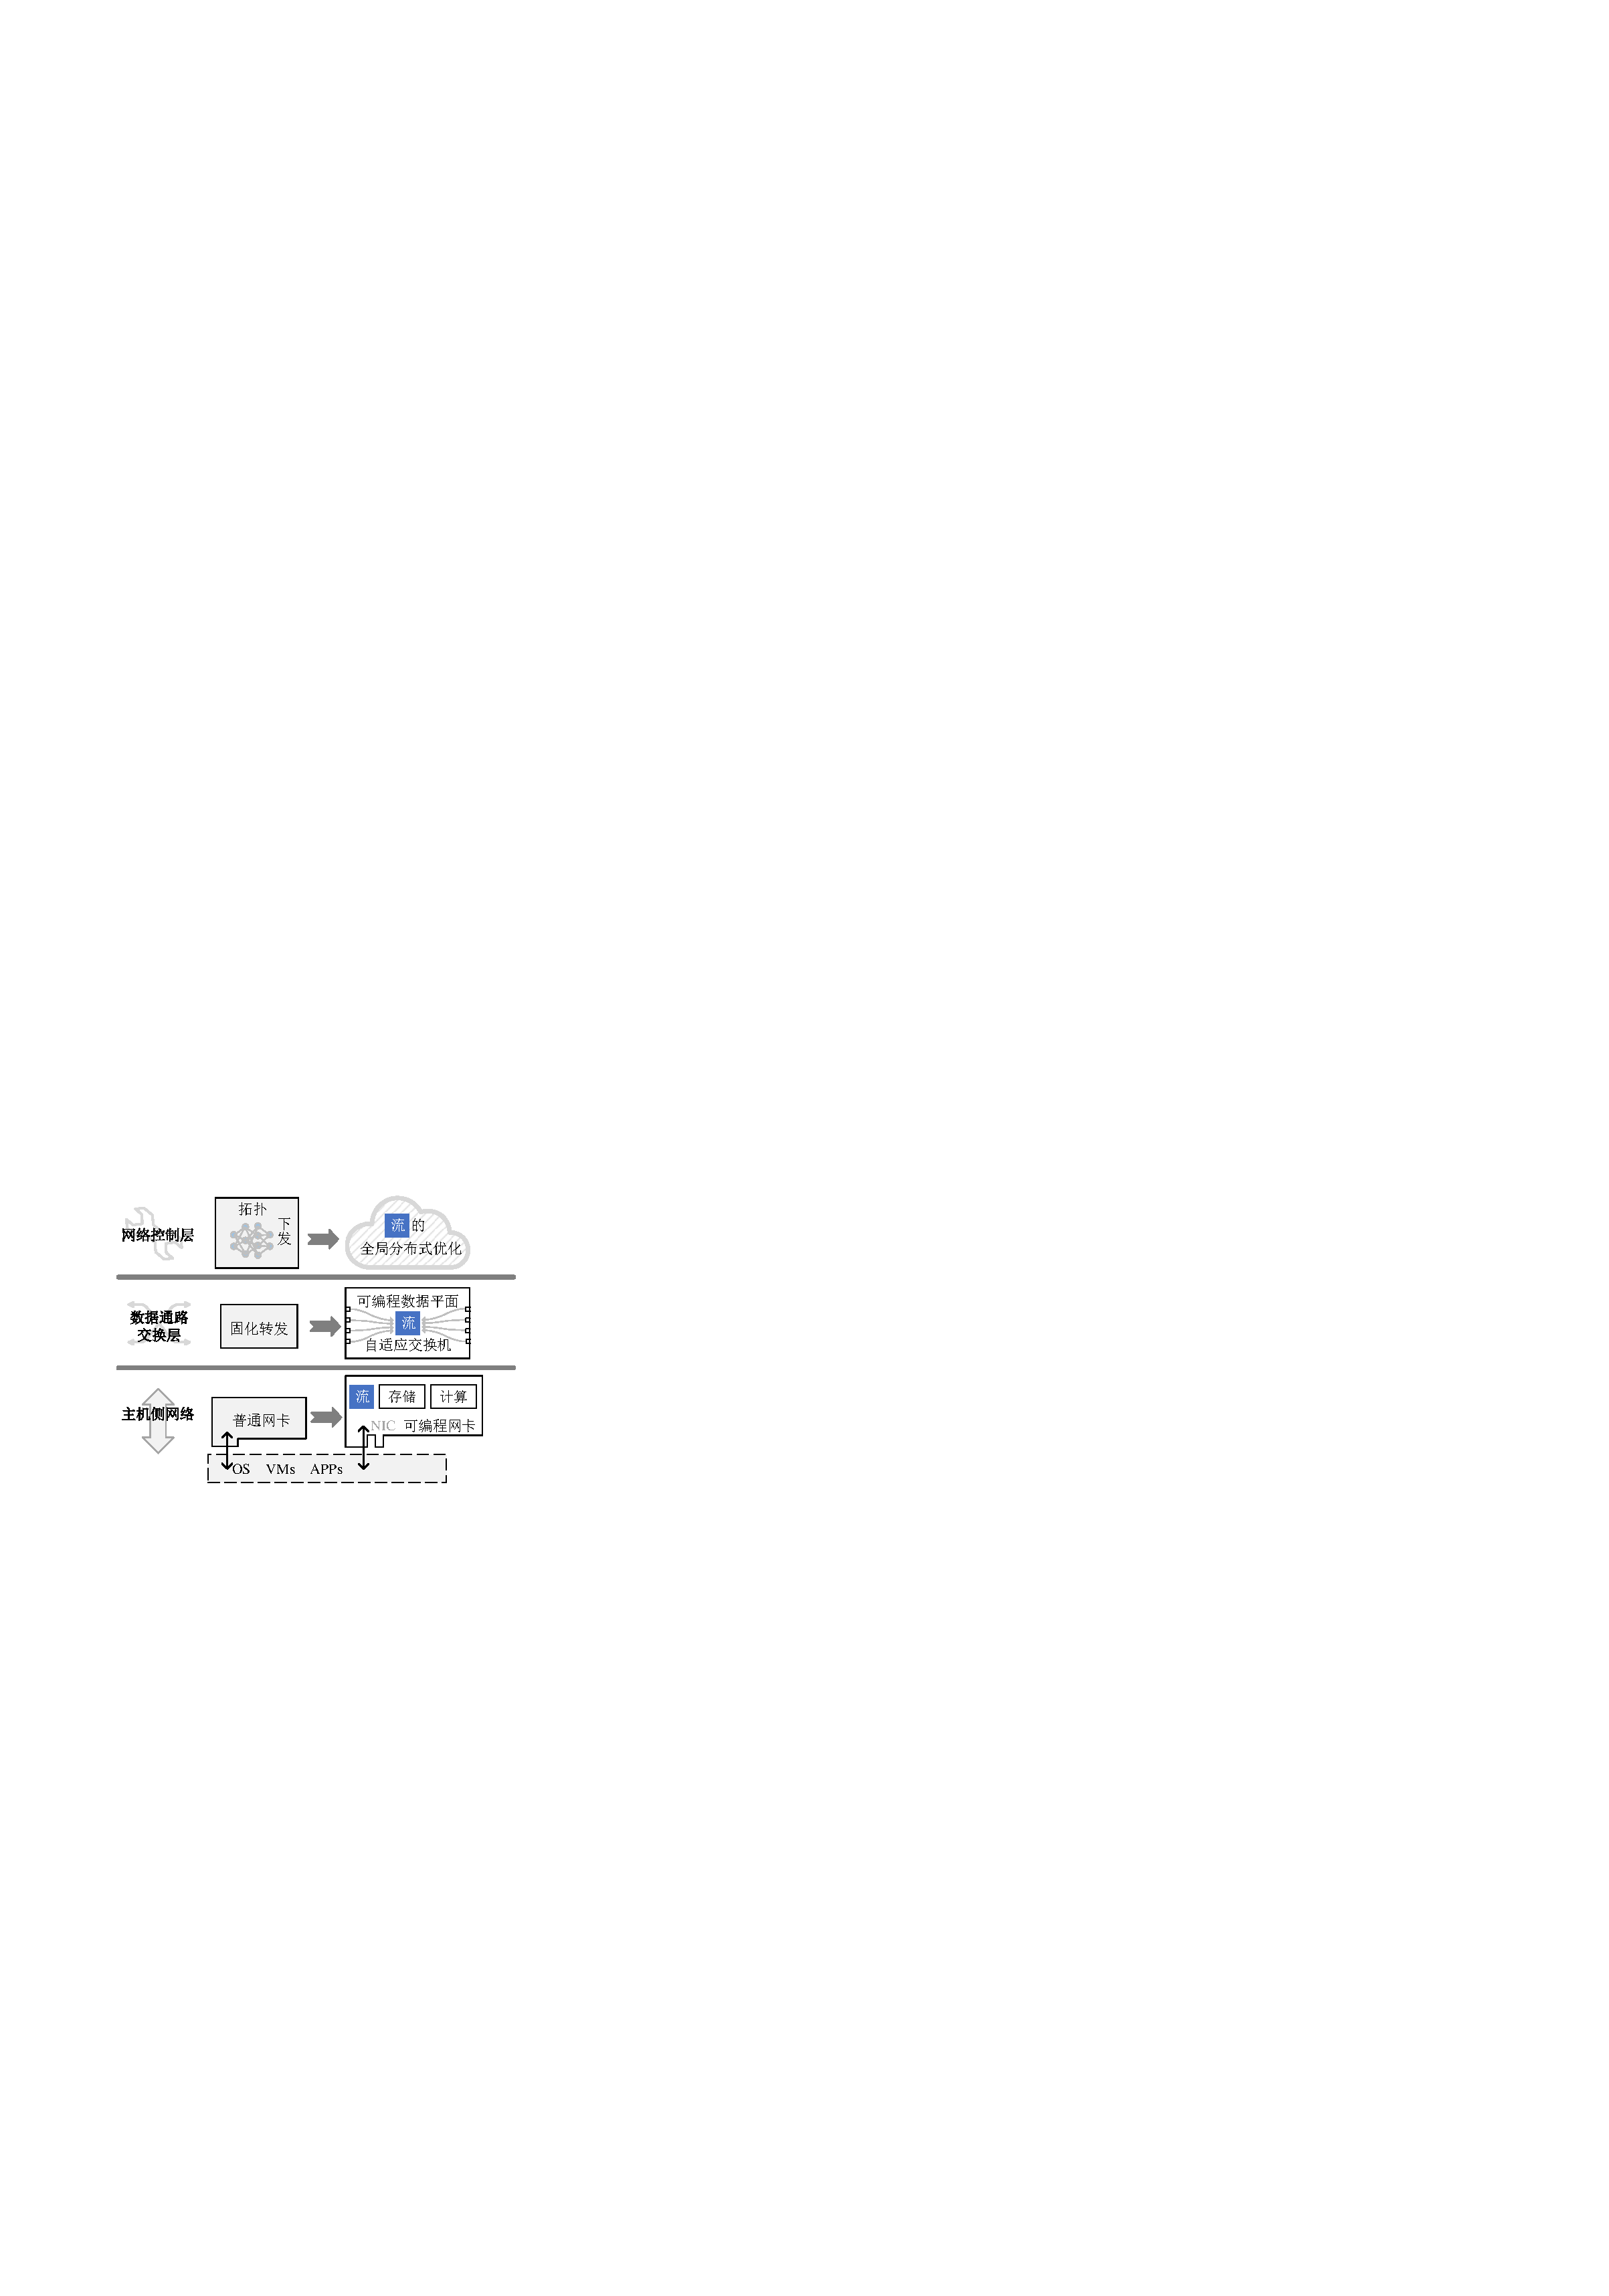
\includegraphics[scale=1]{proghardwarePDParcs.pdf}
	\caption{基于可编程硬件的SDN数据平面研究框架} \label{fig:proghardwarePDParcs}
\end{figure}







1)研究可编程设备加速主机侧网络方法

本文提出利用基于FPGA的智能网卡卸载操作系统内部分网络功能,达到扩展网络接入层的性能的目的。探讨了不同场景下网络功能的构成,分析并提出一种基于可编程硬件的流式计算模型(Data-Computing,DC抽象)。本文将服务器网络功能任务中时间敏感型和计算密集型功能通过合理转换卸载到网卡的FPGA可编程器件中。本文通过网络流量捕获,统计分析和回放的一系列功能场景,展示出在满足网络功能不受改变的前提下,利用基于FPGA的智能网卡可以有效提升服务器的网络性能、时延和效率。

2)研究可编程设备加速网络硬件交换层方法

本文提出一种硬件异构型的可编程网络数据平面架构,将FPGA与ASIC交换芯片有机结合,增强ASIC处理报文的灵活性,同时满足高吞吐的性能需求。论文设计了ASIC面向可编程硬件的扩展接口。交换芯片将数据包头拆分并通过高速数据互联载体发送给FPGA,利用FPGA可重配特性实现完全可编程的包头处理;同时,本文基于DC抽象,将网络随路计算(network-centric computing)模式引入可编程网络体系架构;本文通过分析流量模型在FPGA中设计了一种并行化处理单元,在资源消耗可控的前提下大规模提高系统的可扩展性能;另外本文提出了一套基于可编程硬件混合网络架构的软件定义语言编程框架,实现了软件定义需求和可编程硬抽象层分离,以及针对底层数据平面的一种高效自适应的并行单元流分配算法,可以稳定实时地保障系统交换层的高性能。

3)SDN硬件流表可扩展性研究

由可编程网卡和交换机组成的数据平面内,最重要的资源是流表资源。本文从SDN网络全局视野出发,着手解决流表资源匮乏的问题。本文分析不同的流量规模和特征,以及系统多模块之间的互联协议,提出一种转发设备节点之间的流表共享机制,实现了在流量突发的情形下,保证数据平面稳定性,降低SDN系统控制通道拥塞、失效风险,缓解流表溢出导致转发性能骤降的现象。


\BiSection{关键科学问题}{Challenges}\label{chap13}

1)精度高、性能可扩展性强的网络流量功能卸载方法

面对当前数据量庞大复杂的操作系统网络环境,业界一般会使用专门的软件传输加速工具库(例如,DPDK\citeup{dpdk}),也会使用到例如SR-IOV\citeup{sriov}的专有硬件加速。新一代的网卡还会支持VXLAN、GENEVE等封装技术的卸载,同时基于硬件的远距离直接内存访问(RDMA\citeup{rdma,roce})技术大有取代TCP协议栈的趋势。然而这些基于固定转发平面的卸载技术只能将虚拟化的转发层或者TOE(TCP Offloading Engine\citeup{microsofttcpoffload})卸载下去得到硬件加速,一些基于随路流量的有状态计算、并行计算以及灵活的流量工程却依然难以享受硬件加速带来的优势。目前基于FPGA硬件可编程网卡同时提供了高性能收发和足够强大的灵活性已经可以满足主机侧网络的性能需求,为更复杂功能的卸载提供了有力支持\citeup{alveo250,netfpgaabout}。如何利用可编程网卡实现高精度、高性能保障的网络功能硬件卸载,并且提出网络功能抽象、合理部署、合理划分任务是本文要解决的第一个问题。

2)高资源利用率的高性能硬件可编程数据平面设计方法

在云、服务器--客户端的计算网络体系结构下,由于新兴的内容应用(社交,虚拟/增强,混合现实)以及工业网络应用(移动性,大数据,机器学习)使得网络追求高的实时性、可扩展性。网络设备功能多样性随着数据中心、边缘设备的发展而壮大,因此学界对交换层、核心网场景快速创建灵活解决方案的需求也愈发强烈。可编程数据平面交换机拥有很高的灵活性,可以快速重新定义新的数据包处理协议,为应对新形态网络发展提供了良好前景。其三类典型设计架构但目前都存在缺陷:1)软件交换机性能普遍低下,2)基于ASIC的交换机无法拥有完全可编程性,3)基于FPGA的交换机资源有限,交换性能无法满足业界需求。因此本文第二个研究问题:如何设计一种同时兼顾转发性能和可编程能力的交换设备?如何利用现有设备优势,对其做最小改动以满足设计?如何实现高资源利用率、高灵活性的高性能硬件可编程数据平面设计方法?

3)流表关键资源的全局优化方法

网络数据包的转发动作依赖于数据平面内查找表的匹配结果,SDN架构下亦是如。在此基础上交换机内还增加了多种匹配域、多级流表结构,绝大多数平台中都视转发表为最核心以及成本占用最大的模块。基于硬件的高性能TCAM\citeup{katta2014infinite}(三态内容地址查找表)拥有单周期流水、掩码匹配等优秀性能,但昂贵的价格使得用户无法购置容量足够大的表\citeup{kuzniar2015you},因此交换机内极易发生流表溢出的现象。以OpenFlow协议为代表,一般规定控制器与交换机之间流表安装流程为Reactive模型:交换机收到一条新流首先会上报控制器,随后控制器计算路径并下发流表到数据平面设备。当发生流表溢出现象时,由于Reactive模型需要频繁更替活跃流表内容,这会进一步直接引发控制平面和数据平面之间安全通道的消息风暴,否则会造成丢包或服务任务中断等异常现象。本文第三个研究问题:如何在维持交换机中原有流表容量的前提下,缓解流表溢出所带来的危害?在保持SDN网络平面分离优点的条件下,如何利用其全局化优势高效利用网络设备资源?


\BiSection{主要研究成果}{Reasearch Contributions}\label{chap14}
\begin{figure}[!ht]
	\centering
	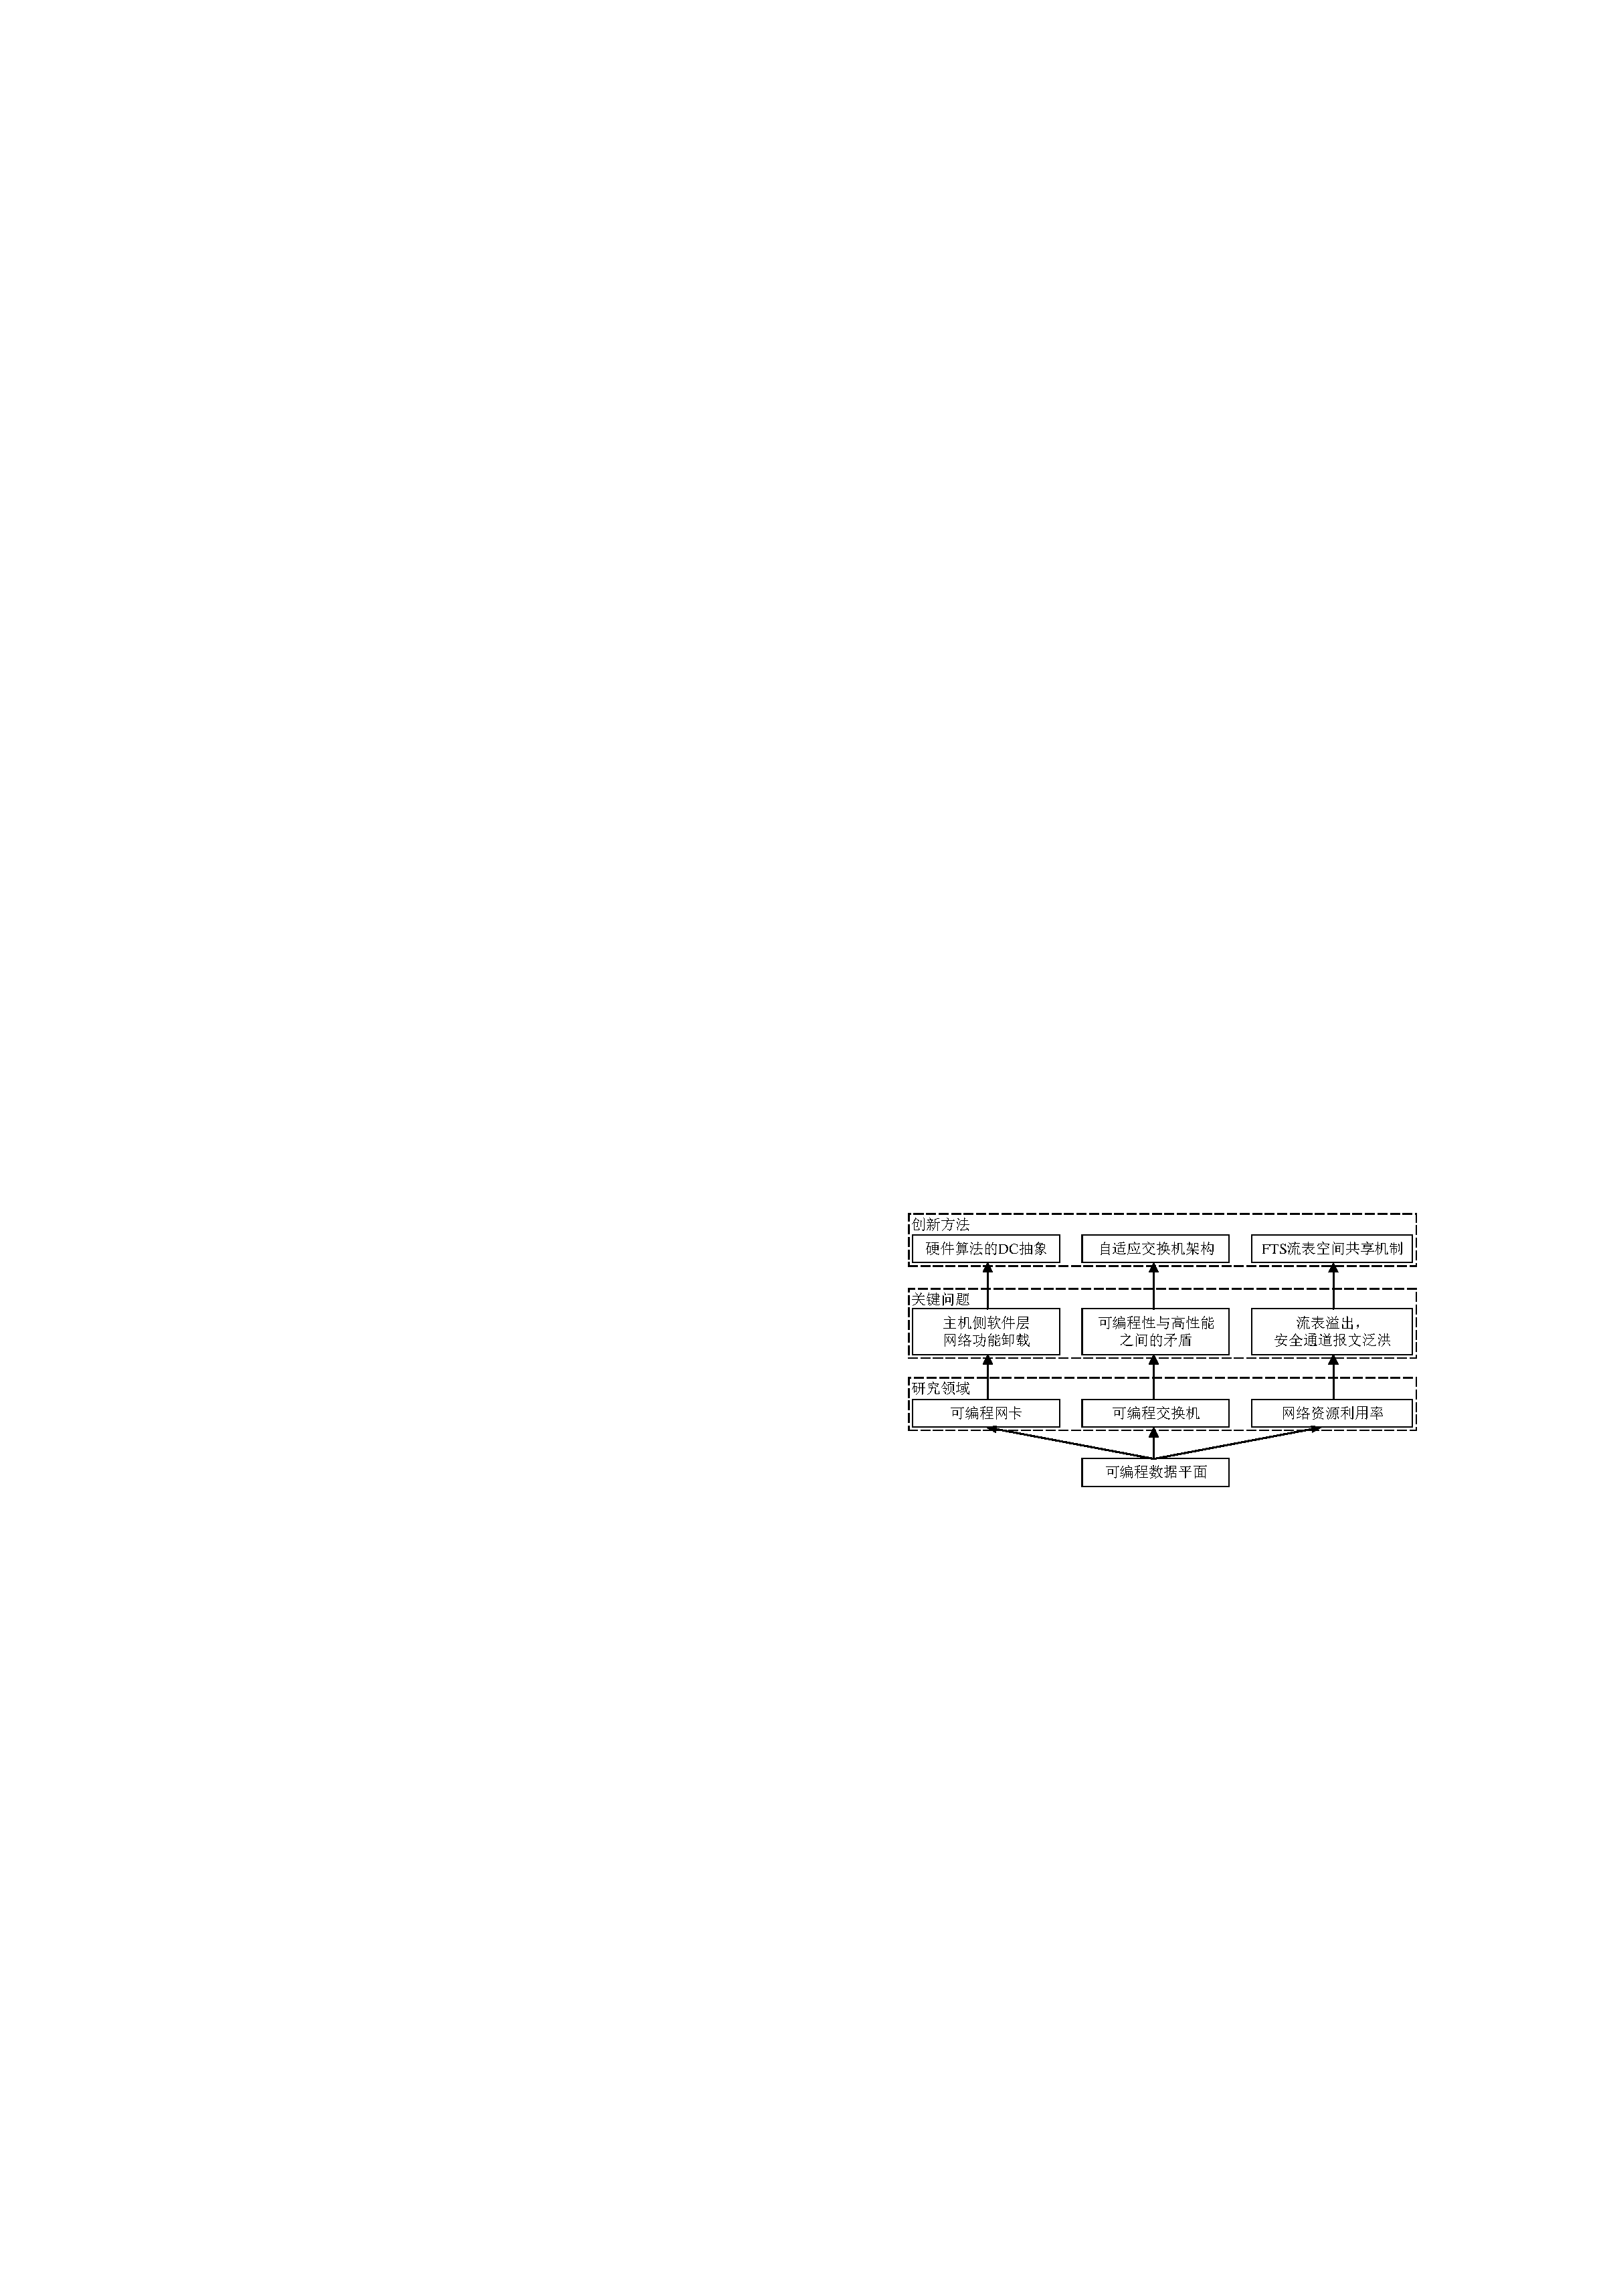
\includegraphics[scale=1]{thesistree.pdf}
	\caption{论文主要研究内容以及成果} \label{fig:thesistree}
\end{figure}

论文针对可编程网卡卸载主机侧网络功能、可编程硬件性能不足以及流表溢出威胁风险大、资源利用率低等问题展开分析和创新方法设计(如图\ref{fig:thesistree})。具体研究成果概况如下:

1)提出了针对流量随路计算的网络功能卸载抽象模型

本文提出一种适用于网络功能硬件卸载的抽象模型:流式计算模型(DATA—COMPUTING, DC抽象)。根据DC抽象,分离软件中适用于硬件加速的繁杂计算,使原本经X86计算架构需要频繁访存的任务,转换到硬件中做流水线式流计算,可在不影响功能的前提下,释放CPU资源、扩展性能、提升系统效率。论文在可编程硬件的网卡中实现了更高精度、更高性能、资源利用率更好的流量捕获-统计-回放应用。实验证明利用可编程硬件能使原有软件性能效提升两个数量级、抖动降低4次方数量级、能源效率提升10倍。


2)提出了FPGA与交换芯片(Switching ASIC)结合的自适应交换机架构

本文提出一种高性能的可重配交换层数据平面架构:自适应交换结构(Adaptive Switch, AS)。通过FPGA与交换芯片联合设计的思想,AS架构可同时提供FPGA的高灵活性与交换芯片的强大性能。论文在前述硬件设计模型的基础上,继续研究硬件逻辑高度并行的性能大规模扩展方法。为了保证FPGA低资源消耗,论文设计了一种基于硬件的灵活负载均衡和资源分配机制。AS架构解决了FPGA性能差与资源少的限制、增强了网络芯片的可编程能力。论文将目前基于FPGA的可编程数据平面性能提升到8Tbps\footnote{当前的研究性能约为100Gbps。}。



3)提出了一种针对流表资源不足场景下的网络内流表共享机制

对于网络转发层核心流表资源不足的问题,本文提出一种全局流表共享方法(Flow Table Sharing, FTS)。本文分析目前OpenFlow协议中有关Table-Miss(流表缺失状态)的处理过程,论证了单纯依靠增加流表容量的方案,并不能使流表溢出的概率降低为零。FTS通过通过增强数据平面自主性等方法,使得新的Table-Miss机制能实现对原先受影响的转发流量RTT时间和安全通道消息风暴数量的优化均达到至少2个数量级,并且能够容易回退、向下兼容现阶段的传统方案。


\BiSection{论文组织结构}{Organization of the Thesis}\label{chap15}

本文的组织结构安排如下:

第\ref{chap1}章为绪论,主要讨论研究背景以及总述全文。

第\ref{sec:pdpintro}章为相关工作综述,分析可编程网络硬件的发展方向、目前研究所面临的挑战。

第\ref{chap3}章论述可编程硬件在主机侧网络环境下的增强作用,使用流量捕获、统计与回放的例子,体现其在提高任务时间精度和资源效率等方面的优势。

第\ref{chap4}章论述一种FPGA与交换芯片相结合的自适应交换架构,在其拥有灵活的可编程能力的同时,处理吞吐性能显著提升。

第\ref{chap5}章主要对网络数据平面内的流表资源做可扩展研究,提出一种全局优化方法来改善流表溢出带来的安全性风险。

第\ref{chap6}章总结全文工作,并展望未来研究方向。








































%-----------------------------------------------------------------------------------------
%\BiSection{为什么用 \LaTeX}{Why}
%
%虽然论文排版是一项基本技能,但是从实际情况看,同学们经常被各种格式整得晕头转向。加之 Word 排版不够美观,版本管理麻烦,排版效率低下,因此开发 \LaTeX{} 论文模板非常重要。国际上许多著名的出版机构和学术期刊都有自己的 \LaTeX{} 模板,国内外许多高效也有自己的硕博论文 \LaTeX{} 模板。事实上,\LaTeX{} 已经成为科技出版行业的国际标准,特别是数学、物理、计算机和电子信息学科。
%
%采用 \LaTeX{} 排版主要有以下优点:
%\begin{enumerate}
%	\item 排版质量高:主要体现在对版面尺寸的严格控制,对字距、行距和段距等间距的松紧适度掌握,对数学公式的精细设计,对插图和表格的灵活处理,对代码和算法的优美呈现,等等。
%	\item 安全稳定:自发布以来 \TeX{} 和 \LaTeX{} 没有发现系统漏洞,不会出现死机或者系统崩溃而导致编写的内容来不及保存。
%	\item 灵活方便:\LaTeX{} 的源文件是纯文本文件,文件大小比 Word 小很多,不会因为文容的增加而导致文档打开、编辑、保存和关闭等操作变慢。因为 \LaTeX{} 在编译时才将所有源文件和图表汇总,故撰写内容时可以随意增删章节和图表。并且和大部分程序设计语言一样,\LaTeX{} 具有注释功能,作者可以在源文件任何地方添加注释,而不会影响最终生成的文档。
%	\item 格式和内容分离:\LaTeX{} 将文档格式和文档内容分开处理,作者只要选择合适的模板,就可专心致志地撰写文档内容,文档的格式细节则由 \LaTeX{} 模板统一规划设置。特别是文献管理能力非常强大,这给撰写像博士论文一样需要大量引用参考文献的文档提供了很大便利。
%	\item 免费开源:\LaTeX{} 软件完全免费,源代码也全部公开,并且相应的配套软件也都采用开源的方式。
%\end{enumerate}
%
%无论你是因为羡慕 \LaTeX{} 漂亮的输出结果,还是因为要给学术期刊投稿而被逼上梁山,都不得不面对这样一个事实:\LaTeX{} 是一种并不简单的排版软件,不可能只点点鼠标就弄好一篇漂亮的文章。还得拿出点搞研究的精神,通过不断练习,才能编排出整齐漂亮的论文。一旦你掌握了如何使用 \LaTeX{} 撰写出精美漂亮的论文时,你会发现你的决定是明智的,你的投入是值得的。
%
%%=========================================================================================
%\BiSection{怎样用 \LaTeX}{How} 
%
%本模板在 Windows + TeXLive2016 + Texsdudio 平台下开发,采用 XeLaTex 编译。虽然之前也开发过一个基于 CTeX 的模板,但是经过多方面比较发现 TeXLive+XeLaTex 处理中文更好,所以基于 CTeX 的模板没有共享。
%
%{\color{red}本模板不能在 CTeX 软件下使用,必须采用 TeXLive,并且编译方式是 XeLaTeX。TeXLive 每年更新一个版本,我用的是 TeXLive2016。文本编辑器可以根据自己的喜好选用,我用的是 Texsdudio,这款开源软件非常不错,推荐大家使用。}
%
%本模板的源文件通过主目录下的 main.tex 统一管理,setup 文件夹中存放格式定义和封面、摘要、目录等内容,body 文件夹中存放论文正文章节的源文件,appendix 文件夹中存放附录、致谢和声明等内容。
%
%本模板只提供论文的格式定义,不提供 \LaTeX{} 的详细使用方法。%所以只回复和论文格式相关的问题,不解答具体的排版方法和技巧。
%因为 \LaTeX{} 的资源非常丰富,大家可以在网上查找资料和并参与讨论,这样学习效率更高。我关注的两个网站是:\url{http://bbs.ctex.org/forum.php} 和 \url{http://www.latexstudio.net};参考的两本书是 ``The Not So Short Introduction to \LaTeXe'' 和 ``LaTeX2e完全学习手册''。
